\documentclass[runningheads]{llncs}

\usepackage{graphicx}
\usepackage{url}
\usepackage{hyperref}
\usepackage{float}

\makeatletter
\newcommand{\printfnsymbol}[1]{%
  \textsuperscript{\@fnsymbol{#1}}%
}
\makeatother

\begin{document}

\title{Species Recommendation using Machine Learning - GeoLifeCLEF 2019}

\author{Nanda H Krishna \inst{1}\thanks{These authors contributed equally.} \and Praveen Kumar R \inst{1}\printfnsymbol{1} \and
Ram Kaushik R \inst{1}\printfnsymbol{1} \and P Mirunalini \inst{1} \and Chandrabose Aravindan \inst{1} \and S M Jaisakthi \inst{2}}

\institute{Department of Computer Science and Engineering, SSN College of Engineering, Kalavakkam, Chennai, India \\
\and
School of Computer Science and Engineering, VIT University, Vellore, India \\
\email{\{nanda17093, praveenkumar17114, ramkaushik17125\}@cse.ssn.edu.in} \\
\email{\{miruna, aravindanc\}@ssn.edu.in}, 
\email{jaisakthi.murugaiyan@vit.ac.in}
}

\authorrunning{ }
\titlerunning{ }
\pagenumbering{gobble}
\maketitle

\begin{abstract}
Prediction of the species present at a location is useful for understanding biodiversity and for the purpose of conservation. The objective of the GeoLifeCLEF 2019 Challenge is to build a species recommendation system based on location and Environmental Variables (EVs). In this paper, we discuss different approaches to predict the most probable species based on location and EV values, using Machine Learning. We first developed purely spatial models which took only the spatial coordinates as inputs. We then built models that took both the spatial coordinates and EV values as inputs. For our runs, we mainly used Artificial Neural Networks and the XGBoost framework. Our team achieved a maximum Top30 score of 0.1342 in the test phase, with an XGBoost-based model.

\keywords{Species Recommendation \and Environmental Variables \and Machine Learning \and XGBoost \and ANN}
\end{abstract}

\section{Introduction}
The prediction of the species present at a location based on spatial and environmental parameters is of great use in understanding biodiversity. It greatly reduces efforts required to collect and analyse data, and allows for more research on the effects of climate change, species invasion and other phenomena on the biodiversity of a region.
\newline 
\newline 
\noindent With the goal of setting up robust information systems relying on automatic identification and understanding of living organisms, the LifeCLEF 2019 challenges \cite{lifeclef2019} were organised. Among these was the GeoLifeCLEF 2019 challenge \cite{geolifeclef2019}, the aim of which was to build a species recommendation system using the given species occurrences and environmental parameters. Environmental Variable (EV) values were given as TIF images, from which the patches for a particular location (latitude and longitude) could be extracted using a Python script \cite{maxgit}. 
\newline
\newline
\noindent Multiple datasets of species occurrences were provided for the contest. One of these was the dataset with trusted occurrences that had an identification confidence score of greater than 0.98, which was derived from the complete occurrences by applying a filter. This dataset, PL\_trusted, contained over 230,000 occurrences and over 1300 distinct species. We used this dataset as it provided the most accurate occurrences with a good confidence score.
\newline
\newline
\noindent The test set for the challenge contained 25000 occurrence IDs for which the species had to be predicted. There were 844 plant species in the test set occurrences, which is a subset of those found in the training sets. Thus, some species present in the training data were non-test species (not present in the test set occurrences).
\newline
\newline
\noindent The evaluation metric for the challenge was Top30, which is the mean of the function scoring 1 if the good species is within the top 30 predicted, or 0 otherwise. The metric is ideal as some tens of plant species usually coexist in the perimeter of the location uncertainty of the occurrences. The Mean Reciprocal Rank (MRR) was used as a secondary metric to enable comparison with previous year results.

\section{Data Preprocessing} 
The occurrences dataset PL\_trusted contained the Latitude, Longitude, Species ID and some other data. From this, we created three different datasets for our usage in different runs, based on the different models we had in mind. 
\subsection{Spatial Data}
We extracted the spatial coordinates and Species ID to create a dataset for training purely spatial models and also a baseline probability-based model. 
\subsection{Spatial and EV Data}
We first created a dataset containing the spatial coordinates and the value of the central pixel for each EV extracted from the EV image patches. Then we created another dataset, containing the spatial coordinates, and the average value of the 16 central pixels extracted from each EV image patch. The values from the image patches were extracted using Python scripts \cite{maxgit}, as tensors. A sample generated from the extractor for a few EVs is shown in Fig. \ref{fig:patch}. The same preprocessing was also applied to the test set during prediction.
\setlength{\abovecaptionskip}{15pt}
\setlength{\belowcaptionskip}{-7pt}
\begin{figure}[htbp]
    \centering
    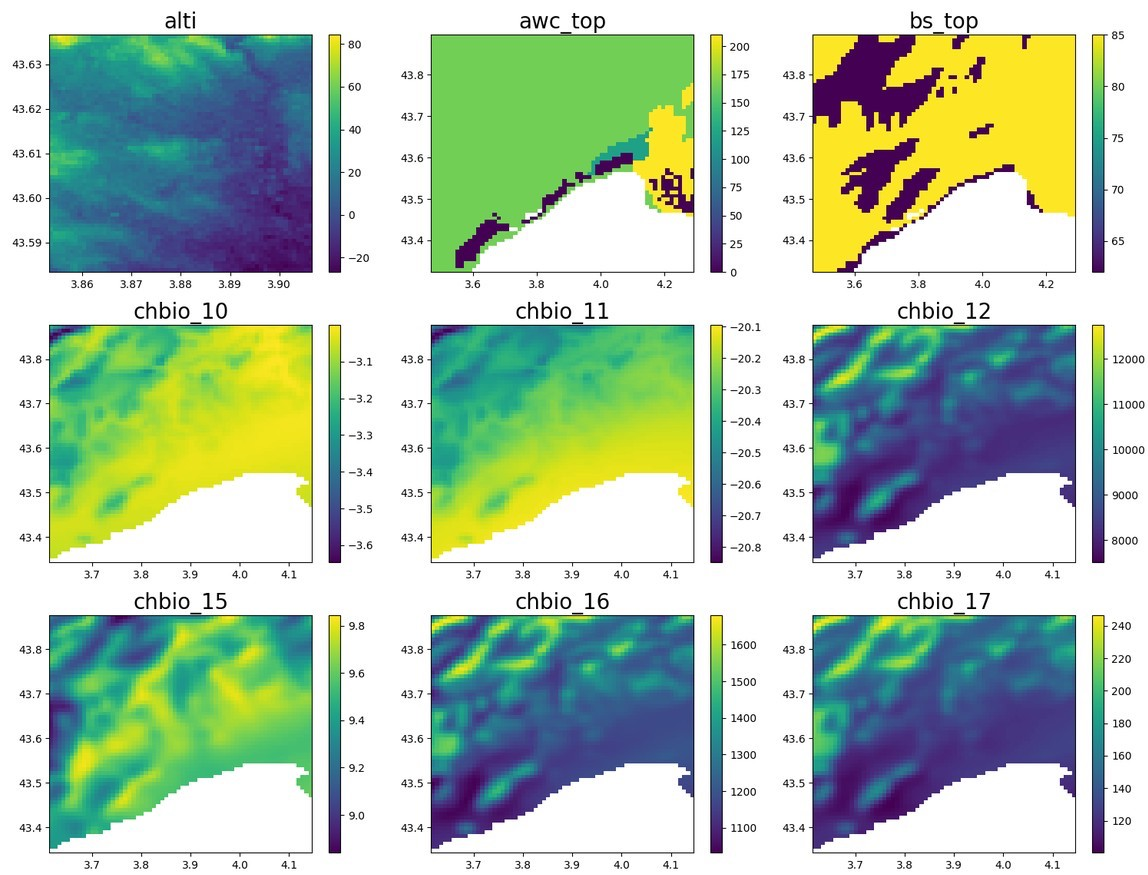
\includegraphics[scale=0.25]{patchs.jpg}
    \caption{Extractor Output Plot}
    \label{fig:patch}
\end{figure}

\section{Methodology}
Our main approaches to this challenge were classifiers based on Artificial Neural Networks using Keras \cite{keras}, the Random Forest Classifier from scikit-learn \cite{scikit-learn} and the XGBoost library \cite{xgboost}.
\subsection{Probability-based Model}
We created this model for our understanding of the species distribution across the whole dataset of occurrences, and submitted it as our baseline approach. We used the occurrences data to obtain the number of occurrences of each individual species, and thus determined their probabilities. The list of species was then sorted in descending order of probabilities, and the non-test species were removed. From this, the top 50 species were chosen. For each test occurrence, the same list of 50 species was assigned in the submission. This run (26821) had a Top30 score of 0.0570.
\subsection{Purely Spatial Models}
The purely spatial models take only the spatial coordinates, that is, the latitude and longitude of the occurrences as inputs, and output a list of probabilities of the species. The predictions for each occurrence were sorted in descending order of probabilities, following which the non-test species were removed. The top 30 species for each occurrence were chosen for the submission. We built purely spatial models using XGBoost, ANNs and Random Forest Classifiers.
\subsubsection{XGBoost:} This model used the XGBoost framework, where we set the parameter $eta$ to 0.1 and the objective function to XGBoost's $multi:softprob$ which is used for multiclass classification. The $num\_round$ parameter in training was set to 1. This run (26988) had a Top30 score of 0.1063. 
\subsubsection{ANN:} We used an Artificial Neural Network developed using the Keras library (Tensorflow backend) for this model. The Sequential model had 5 hidden Dense layers with 256 units and the $relu$ activation function. Two Dropout layers with $rate$ 0.02 were present, one after the first 2 Dense layers and the other after the next 2 Dense layers. The final output layer had the number of units set to the number of species in PL\_trusted, with $softmax$ activation - to predict class probabilities. The model was compiled with $adam$ optimizer and $categorical\_crossentropy$ loss, for 10 epochs and a batch size of 2000. The Top30 score for this run (26875) was 0.0844. The summary of the model is shown in Fig. \ref{fig:ann}.
\setlength{\abovecaptionskip}{15pt}
\setlength{\belowcaptionskip}{-22pt}
\begin{figure}[h!]
  \centering
  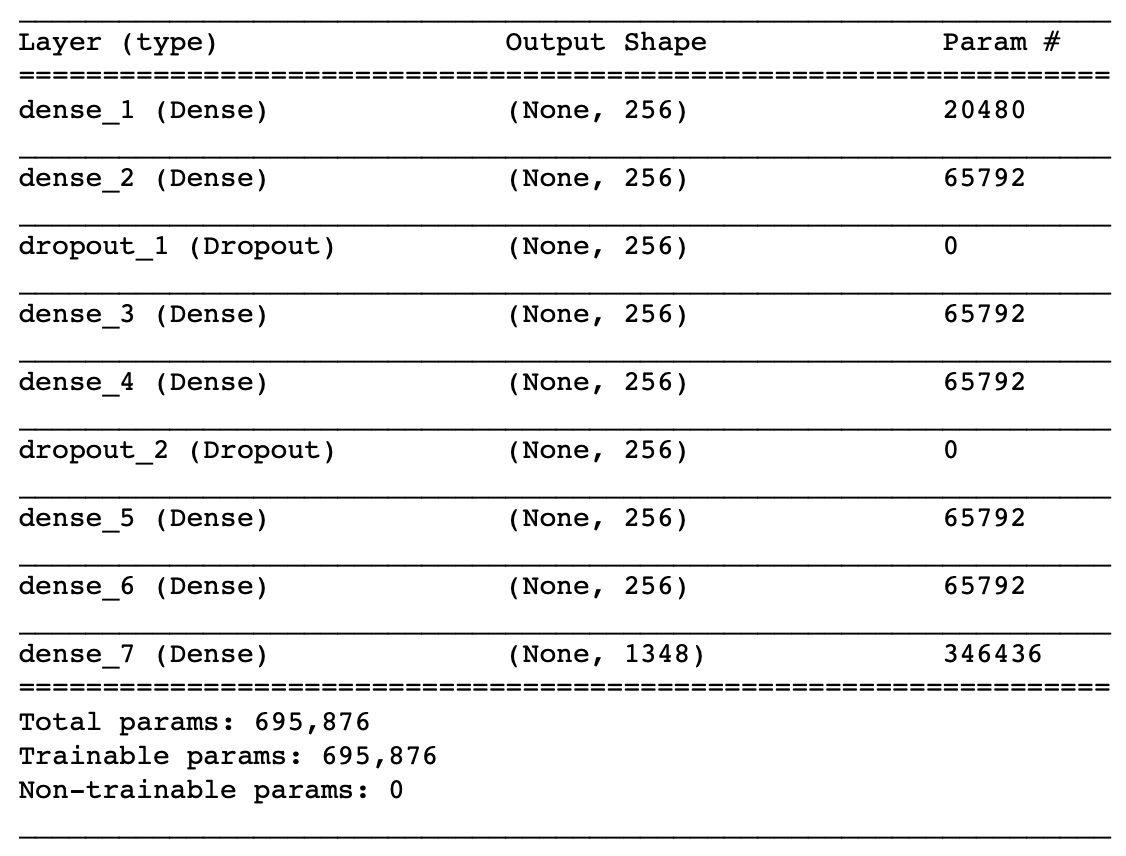
\includegraphics[scale=0.5]{ann.png}
  \caption{ANN Model Summary}
  \label{fig:ann}
\end{figure}
\subsubsection{Random Forest:} This model was built using the in-built RandomForestClassifier in the scikit-learn framework, with $n\_estimators$ set to 10. The Top30 score of this run (27102) was 0.0834.
\subsection{Models Based on Spatial Coordinates and EV Values}
These models had the spatial coordinates and the extracted EV values as their inputs, and were trained to predict species probabilities. We made 8 submissions based on these data, using XGBoost, a Multiple ANNs model and an ANN taking selected features as inputs. In each approach, the non-test species were removed from the list of predictions, and the top 30 species based on probability were chosen to be submitted for each test occurrence.
\subsubsection{XGBoost:} We made 4 submissions (26996, 26997, 27012, 27013) using the XGBoost library. The differences between these runs was the value of the $max\_depth$ parameter of the model, and the dataset used in training. All EV values were used in three runs (26997, 27012, 27013) while all EV values except the categorical feature $clc$ were used in one run (26996). The value of parameter $eta$ was set to 0.1, the objective was set to $multi:softprob$ and the $num\_round$ parameter during training was set to 1 in all these runs. The details of the models can be found in Table \ref{table:xgbev}. It is to be noted that our top scoring submission was achieved with this method (26997), with a Top30 score of 0.1342.
\setlength{\tabcolsep}{6pt}
\begin{table}[]
    \centering
    \setlength{\abovecaptionskip}{25pt}
    \setlength{\belowcaptionskip}{-25pt}
    \begin{tabular}{| c | c | c | c |}
         \hline
         \textbf{ Run } & \textbf{ Extracted EV Values }  & \textbf{ max\_depth } & \textbf{ Top30 Score } \\
         \hline
         26996 & Single Central & None & 0.1288 \\
         \hline
         26997 & Average of 16 Central & None & 0.1342 \\
         \hline
         27012 & Average of 16 Central & 3 & 0.1263 \\
         \hline
         27013 & Single Central & 3 & 0.1273 \\
         \hline
    \end{tabular}
    \caption{XGBoost Models trained on Spatial Coordinates and EV values}
    \label{table:xgbev}
\end{table}
\subsubsection{Multiple ANNs:}
We developed a unique model which consisted of 5 different ANNs. We split the features - spatial coordinates and EV values - into 5 different mutually exclusive and exhaustive groups, each of which was the input to an ANN. The outputs of each ANN were the probabilities of the various species. The output vectors of each ANN, containing the probabilities, were averaged to get the final probability for each species. The architecture of all 5 ANNs was the same as used earlier (refer Fig. \ref{fig:ann}). The only difference is the input dimension, which is based on the group of features sent as inputs to the ANNs. Also, the feature $clc$ was integer encoded before being passed to the ANNs. The features sent to each ANN can be found in Table \ref{table:manns}.
\begin{table}[]
\centering
\setlength{\abovecaptionskip}{20pt}
\setlength{\belowcaptionskip}{-7pt}
\begin{tabular}{|c|c|c|c|c|}
\hline
\textbf{ANN 1} & \textbf{ANN 2} & \textbf{ANN 3} & \textbf{ANN 4} & \textbf{ANN 5} \\ \hline
Latitude & chbio\_10 & chbio\_17 & chbio\_6 & erodi \\
Longitude & chbio\_11 & chbio\_18 & chbio\_7 & etp \\
alti & chbio\_12 & chbio\_19 & chbio\_8 & oc\_top \\
awc\_top & chbio\_13 & chbio\_2 & chbio\_9 & pd\_top \\
bs\_top & chbio\_14 & chbio\_3 & crusting & proxi\_eau\_fast \\
cec\_top & chbio\_15 & chbio\_4 & dgh & text \\
chbio\_1 & chbio\_16 & chbio\_5 & dimp & clc \\ \hline
\end{tabular}
\caption{Groups of Features for each ANN}
\label{table:manns}
\end{table}
\newline
\noindent We made 2 submissions using the Multiple ANNs model (27064, 27067). The first submission (27064) was made based on the dataset with EV values extracted from the central pixel of the patches, and it obtained a Top30 score of 0.1198. The second submission (27067) was made based on the dataset with EV values extracted by averaging the central 16 pixel values, and it obtained a Top30 score of 0.1135.
\subsubsection{Selected Features ANN:}
Another approach we tried was an ANN with selected important features as inputs. The ANN used has an architecture similar to that of the ones used earlier (refer Fig. \ref{fig:ann}) but with different input dimension. We selected what we identified as important features based on data observation and geological knowledge. Thus the features selected as inputs to the ANN were Latitude, Longitude, $alti$, $awc\_top$, $bs\_top$, $chbio\_1$, $chbio\_10$, $chbio\_11$, $chbio\_17$, $chbio\_18$, $chbio\_19$, $chbio\_2$, $chbio\_3$, $erodi$ and $etp$.
\newline
\newline
\noindent Of the 2 submissions made using the Selected Features ANN, one (27069) used the dataset with EV values extracted by averaging the central 16 pixel values of the patches, while the other used the dataset with EV values extracted from the central pixel alone. The Top30 scores of these submissions were 0.1227 and 0.1268 respectively.
\subsection{Other Unsubmitted Methods}
Initially, we had tried to use more advanced methods to approach this problem such as ResNet and Convolutional Neural Networks. We did this because of the great reputation of these Networks to problems such as image classification. However, these runs were highly unsatisfactory and poorer than the rest of our approaches. Thus, we did not submit these runs for evaluation.

\section{Source Code and Computational Resources}
We have uploaded our source code in the form of Jupyter Notebooks to a public GitHub repository\footnote{\url{https://github.com/nandahkrishna/GeoLifeCLEF2019}}. Instructions are provided for installing requirements and using the Notebooks. The resources we used were a 2.6 GHz Intel i7 CPU and an NVIDIA 940M GPU. Our unsubmitted models were trained using a Google Cloud VM instance with 8 CPUs.

\section{Results}
In the GeoLifeCLEF 2019 challenge, our team SSN\_CSE achieved a top submission rank of 6, with a best Top30 score of 0.1342. Overall, we were ranked 3rd. The top rankers were team LIRMM with a best Top30 score of 0.1769 and team SaraSi with 0.1687. The overall results can be seen in Fig. \ref{fig:t30} and on the challenge website \cite{web}.
\begin{figure}[H]
    \centering
    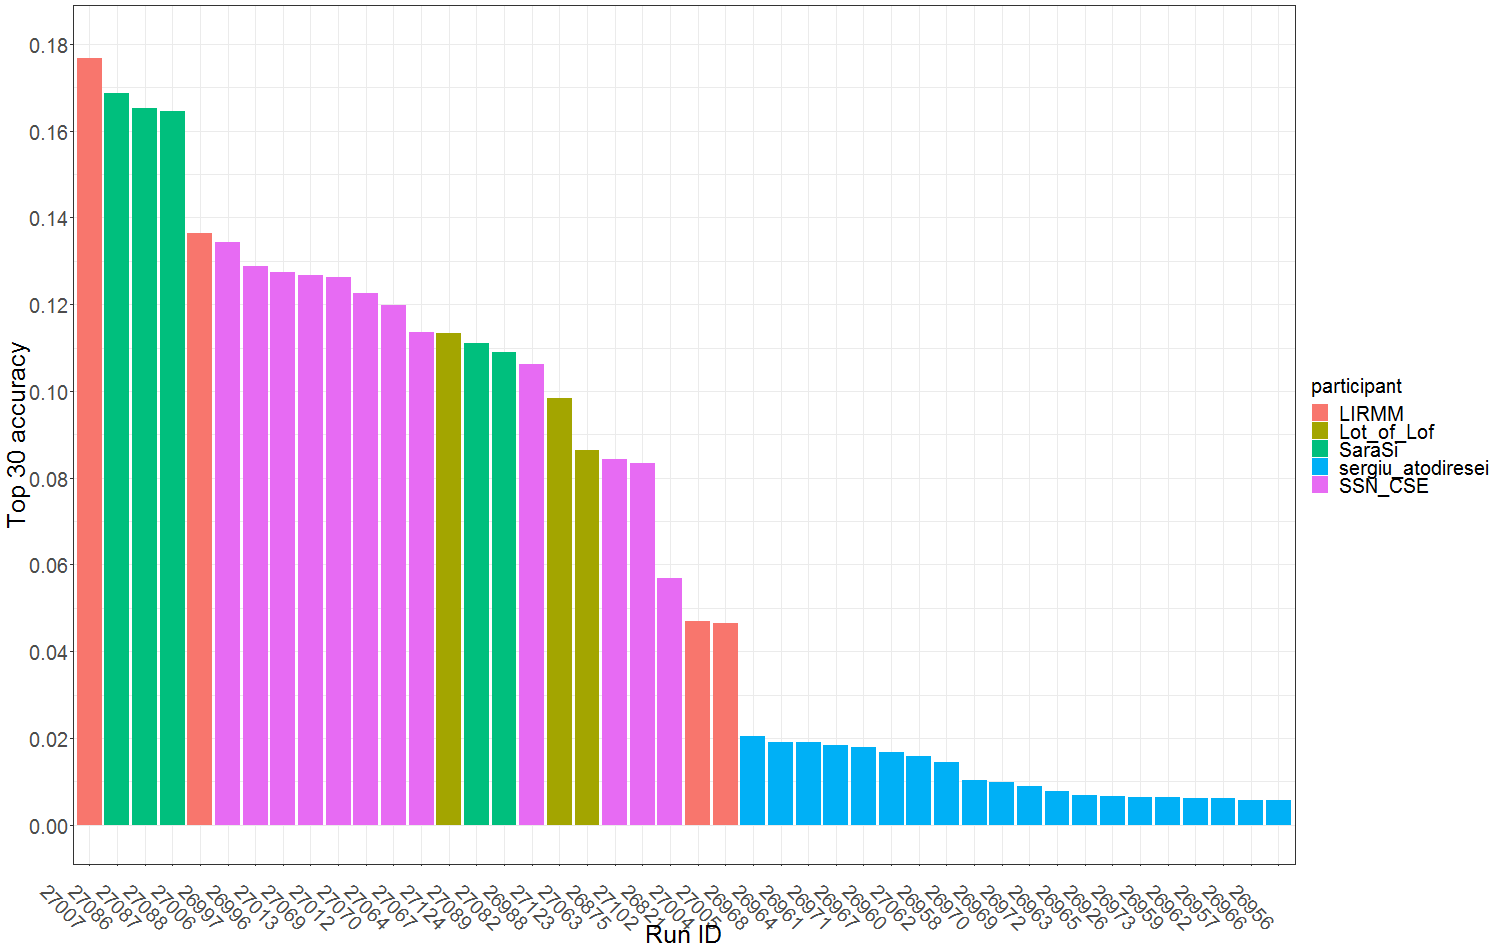
\includegraphics[scale=0.25]{top30.png}
    \setlength{\abovecaptionskip}{15pt}
    \setlength{\belowcaptionskip}{2 pt}
    \caption{Graph showing run-wise Top30 scores}
    \label{fig:t30}
\end{figure}

\section{Conclusion and Future Work}
The overall results of the challenge show the difficulty in building species recommendation systems. We approached this problem using various Machine Learning techniques and evaluated their performance in this task. We thus learnt a great deal about the uses and advantages of these methods. 
\newline
\newline 
\noindent Early on, we found that complex models such as ResNet did not perform greatly in the task. This was shown by the results of last year's edition of the challenge \cite{glc18}. The poor predicting power of our unsubmitted models could be attributed to the curse of dimensionality, vanishing probabilities due to large number of classes, and also the fact that the EV image patches are very different from the traditional photographic images they are generally used for. Even a simple probability-based model and purely spatial models outperformed these models. Purely spatial models did not perform very bad, but models using the EV values greatly outperformed them. The XGBoost models produced good results in last year's edition of the challenge and we observe a repeat of that in our submissions this year, often outperforming ANNs. However, the top submissions involved species co-occurrence models which would have enhanced the predictive power and thus performance in the challenge.
\newline
\newline
\noindent In the future, our aim would be to enhance our current models by hyper-parameter tuning and the incorporation of co-occurrence based data. External data sources and co-occurrence models could help in enhancing the results. We also aim to explore different custom designed Neural Network architectures to improve performance on this task.

\section{Acknowledgements}
We thank SSN College of Engineering for allowing us to use the High Performance Computing Laboratory during our work for this challenge. We thank Dr. M A Rajamamannan (Government Arts College, Coimbatore) for his help in identifying the important features for species recommendation.
\bibliographystyle{splncs04}
\bibliography{ref}
\end{document}
